\chapter{Appendix}

\section{COFW-Images and Fits}
\label{appendix:COFW}

\begin{figure}
	\centering
	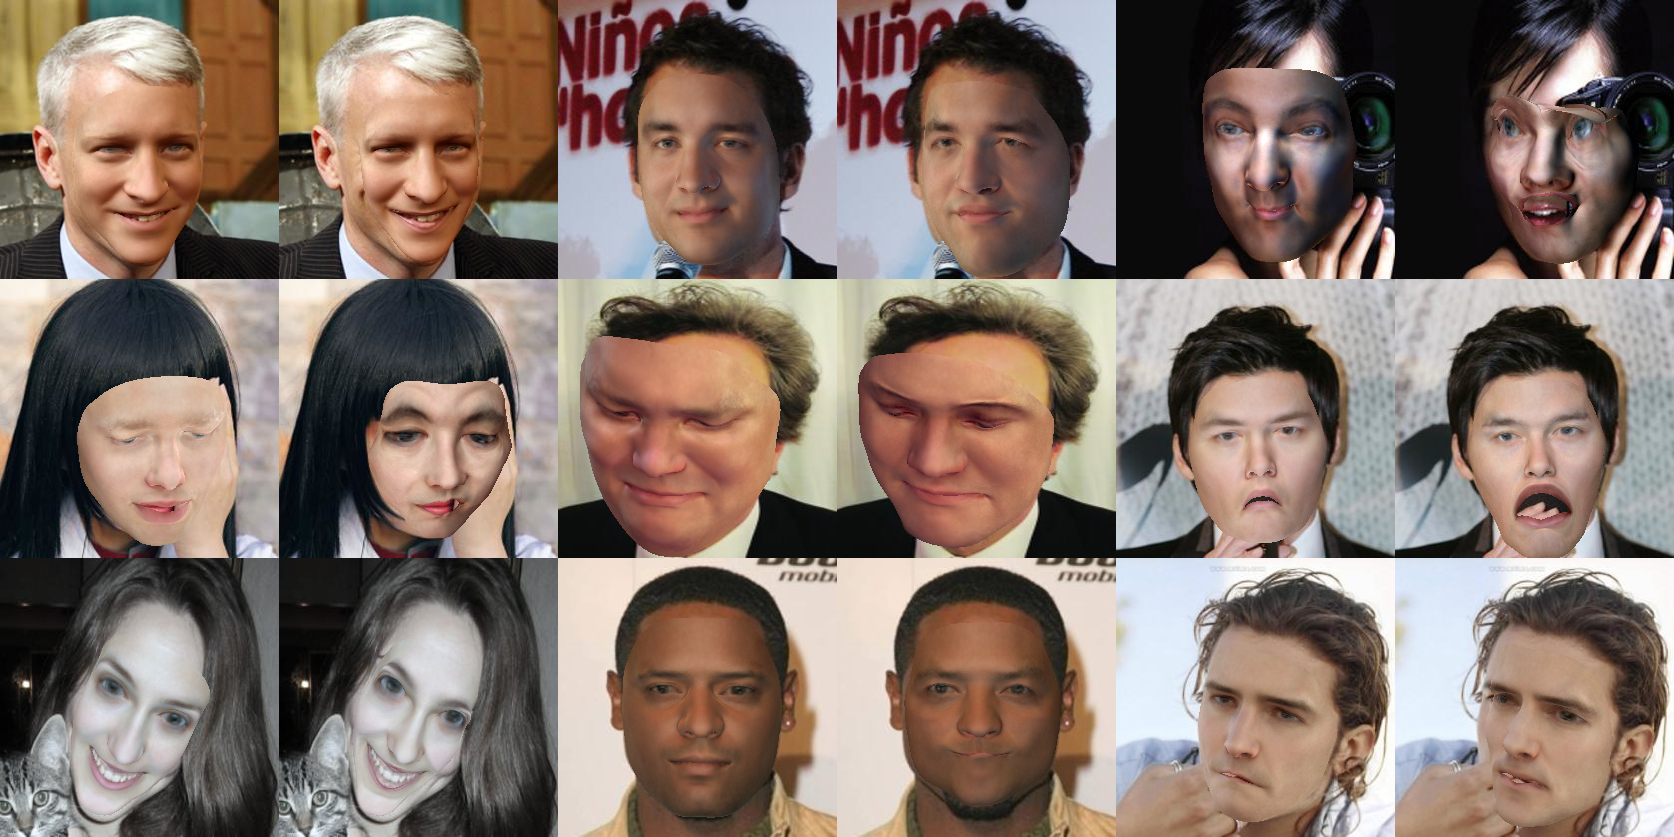
\includegraphics[width=0.9\textwidth]{Figures/appendix/COFW_Fits_Appendix.png}
	\caption{The additional images of Figure \ref{fig:chap2:COFW_Fits}. In each tuple the first plot shows the fit with the mask of egger et al. and the second plot is made with the segmentation of the FCN.}
	\label{fig:chap2:COFW_Fits_Appendix}
\end{figure}

\vspace{3cm}

\section{Datasets other than Hands(which are shown in the thesis)}
\label{appendix:otherDatasets}

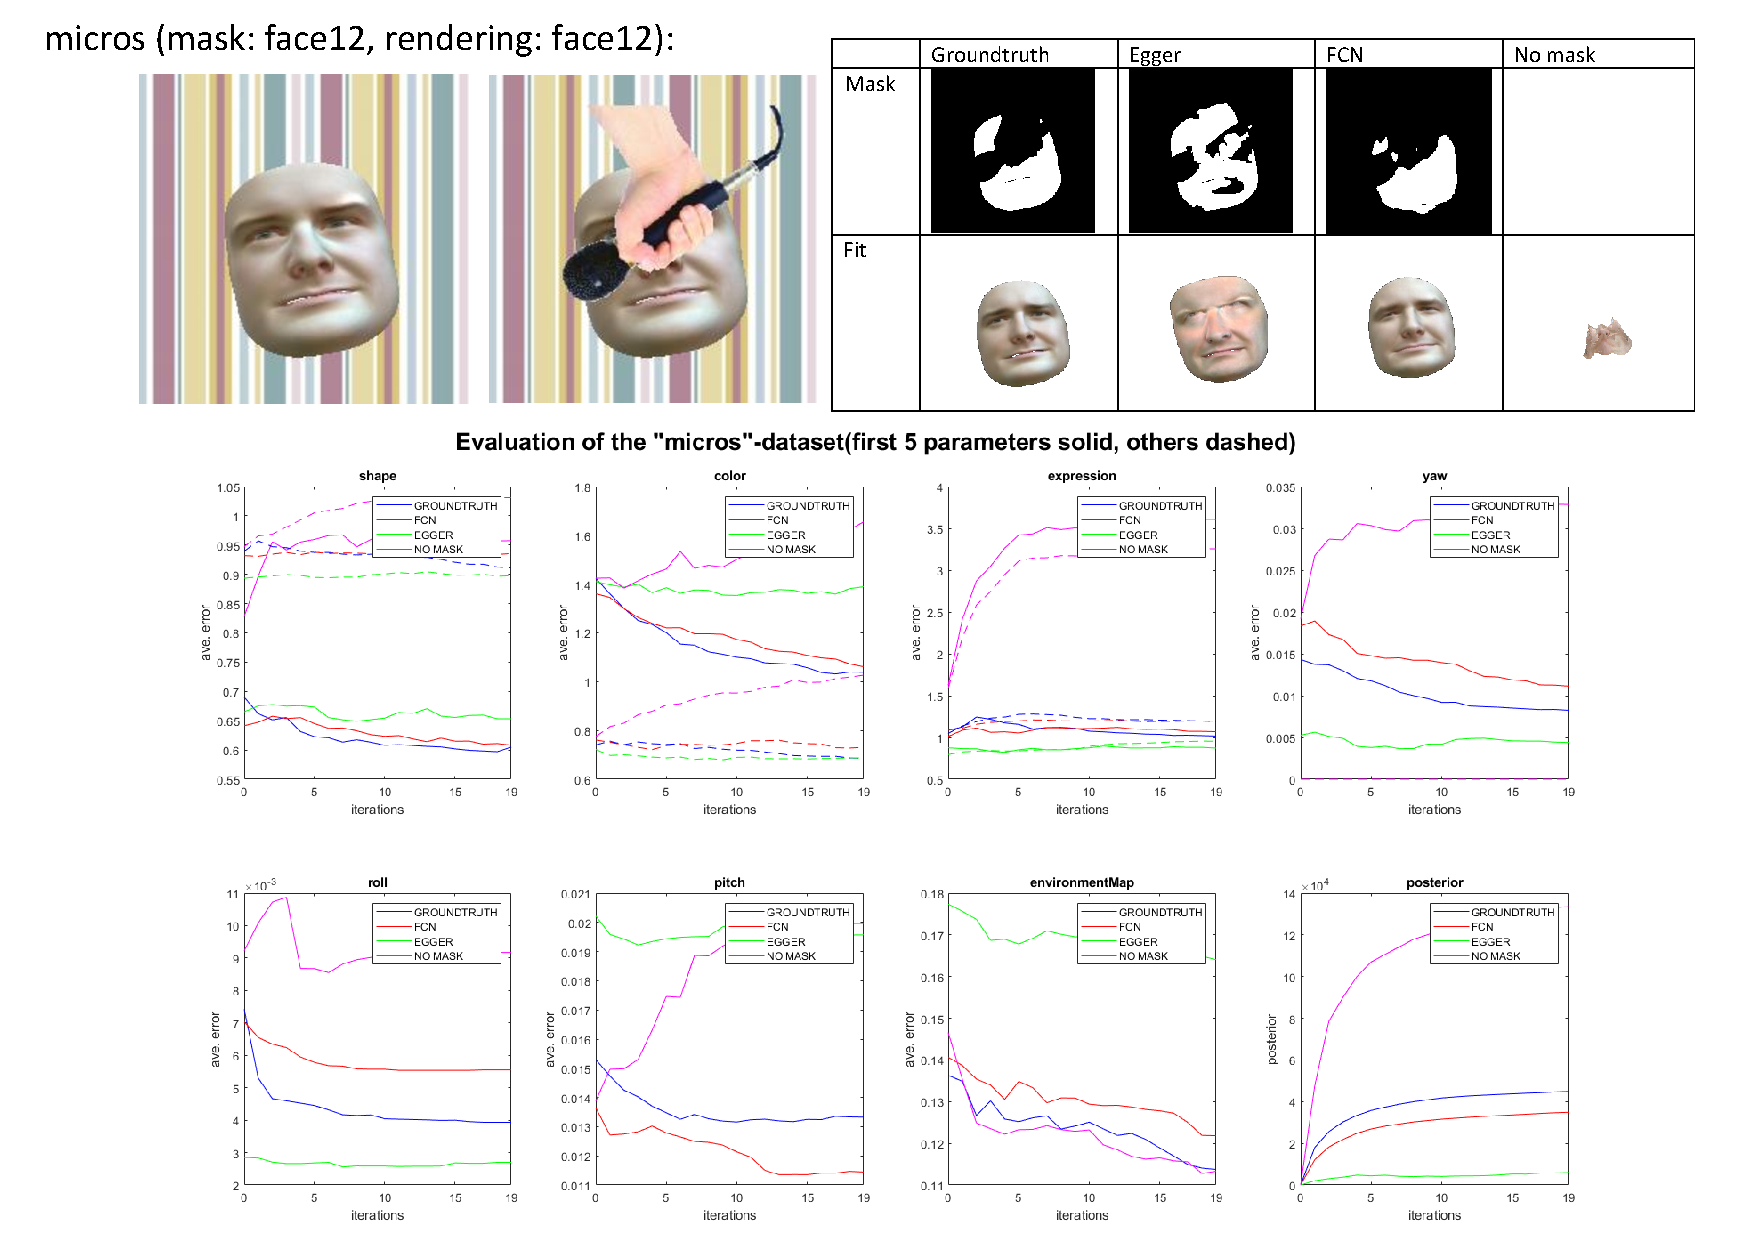
\includepdf[landscape=true,pages={1-16}, angle=180]{Figures/appendix/forAppendix.pdf}

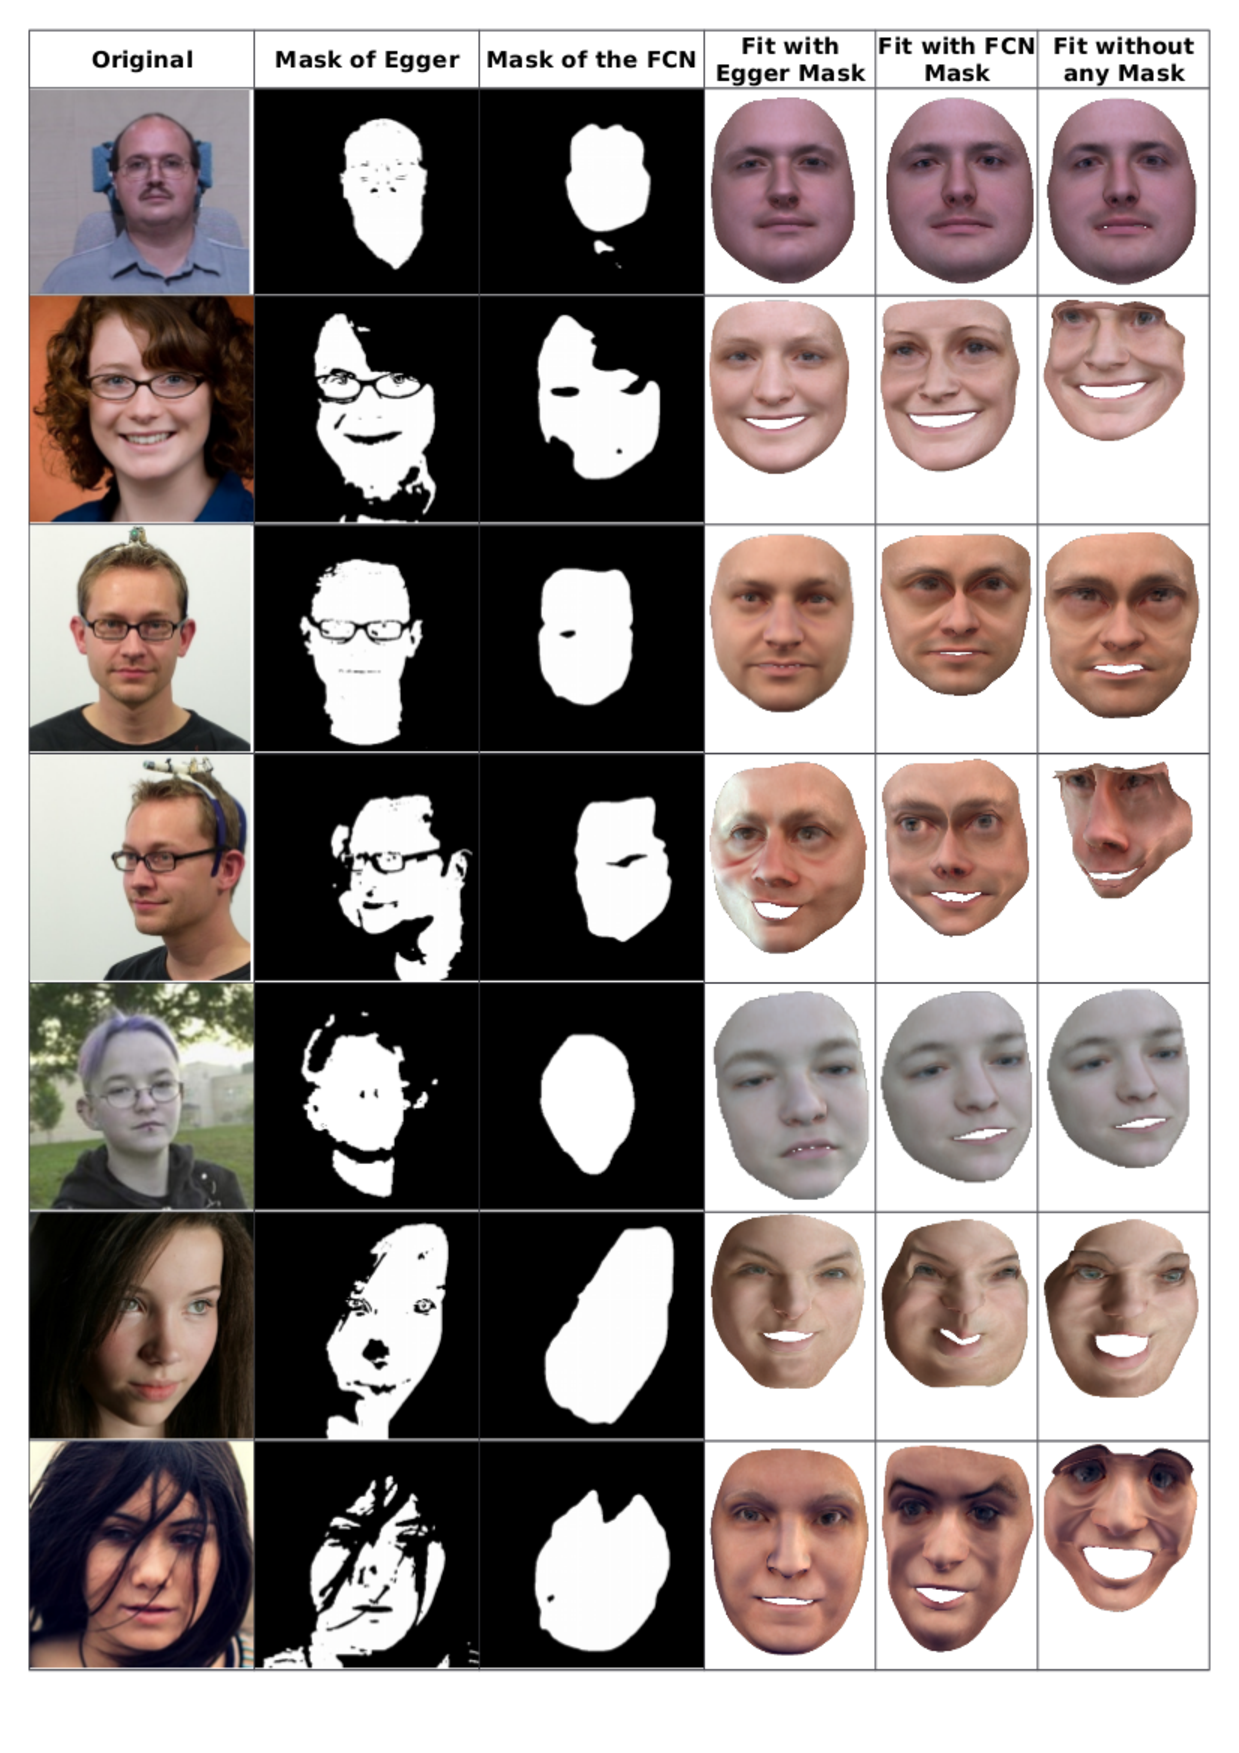
\includegraphics[width=1\textwidth]{Figures/appendix/Real-Life/Real-Life_1.pdf}
\label{appendix:real-world data}
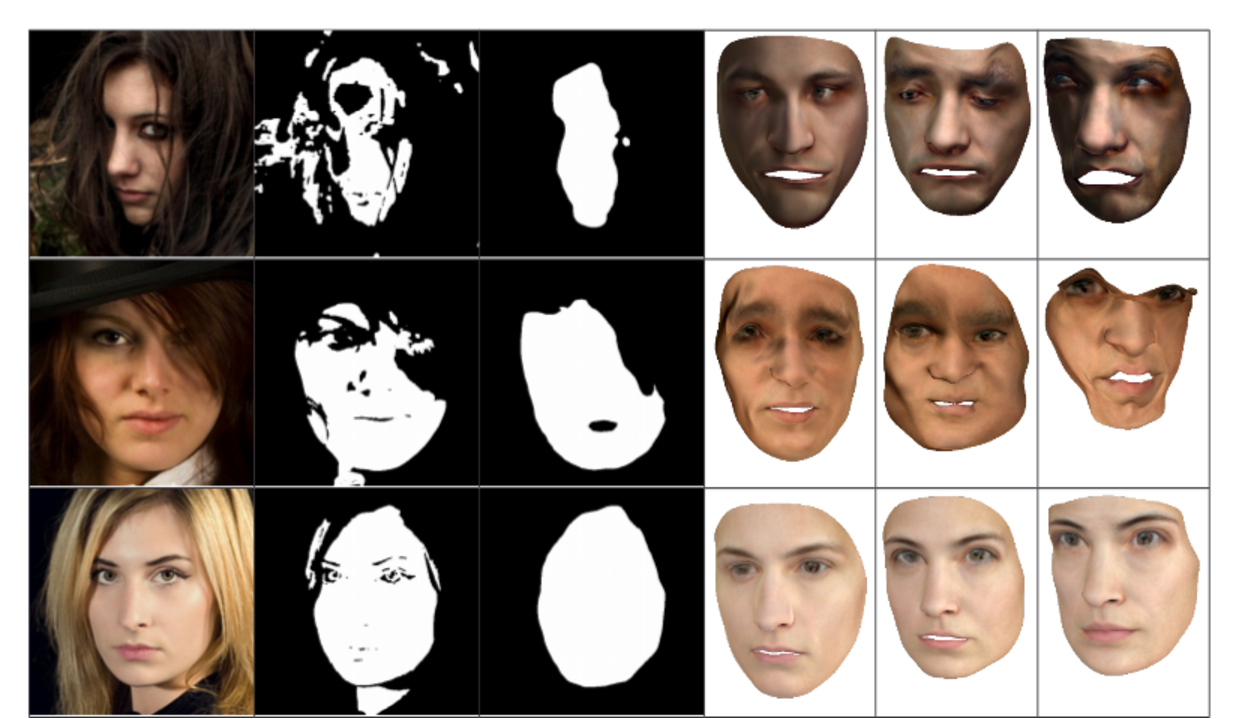
\includegraphics[width=1\textwidth]{Figures/appendix/Real-Life/Real-Life_2.pdf}


\section{Discussion of the Results}
For the synthetic data, a distinction must be made between the occlusions on which the FCN was trained on (hands, micros, glasses) and those unknown to the FCN (random boxes). For known occlusions, the FCN's mask is often more accurate than the one of Egger et al. If these masks are used for fitting, the errors of the parameters ('shape', 'color', 'expression', 'environmentMap') are either very close to those of the fit with the Egger mask, or even better.\\
\\
The random boxes are not recognised by the FCN. The mask is very bad compared to Egger. However, just a few segmented points are enough to get a good fit. Because of the very low false positive rate of the FCN, the fits are comparable to those with the mask of Egger et al. Without occlusion, the masks of the FCN are clearly better than those of Egger. The resulting fits are almost impossible to compare with the naked eye. Due to the Basel Face Model parameters, the fit with the FCN mask is sometimes better than the one with the segmentation of Egger et al.\\
\\
An eye-catching detail is that with the segmentation of Egger et al on the setting with the 'bfm' rendering (on the no occlusion dataset) a very small error of the shape parameter can be achieved. This could be because much more of the face shape is known due to the over-segmentation.

The real life data shows the enormous advantage of Egger. Although the segmentation of the FCN is not bad. The occlusion-aware method of Egger et al can recognise very thin partial coverings such as glasses and separate them from the facial region.


\section{Parametric-Face-Image-Generator}
We extended the Parametric-Face-Image-Generator of Kortylewski et al \cite{parametric}. In our version the option "occlusionMode" in the configuration files can now be set to:
\begin{itemize}[nolistsep]
	\item \textbf{"eyes"}: A circle occludes the picture centered on the pupil centers of the face.
	\item \textbf{"random-1"}: A  hand hides the picture in a random place in a random orientation.
	\item \textbf{"random-2"}: A  microphone hides the picture in a random place in a random orientation.
	\item \textbf{"random"}: A randomly chosen occlusion image hides the picture in a random place.
	\item \textbf{"box"}: A box filled with an arbitrary color hides the image.
	\item \textbf{"box-whiteNoise"}: A box filled with Gaussian white noise hides the image.
	\item \textbf{"box-skinColor"}: Boxes filled with the colour at the tip of the chin hide the image on a random place.
	\item \textbf{"box-[0-100]"}: Boxes filled with a random colour sized that they occlude the specified amount of face pixels.
	\item \textbf{"loop"}: Produces 20 copies of the same image, each with a box occluding 2,4,6,...,40 \% of the face.
	\item \textbf{"texture"}: Fills a randomly placed box with a specified texture image.% specified in the folder 'textures'.
\end{itemize}


\begin{figure}
	\hspace*{\fill}%
	\subbottom[A facial image of the parametric face image generator with all landmarks activated.]{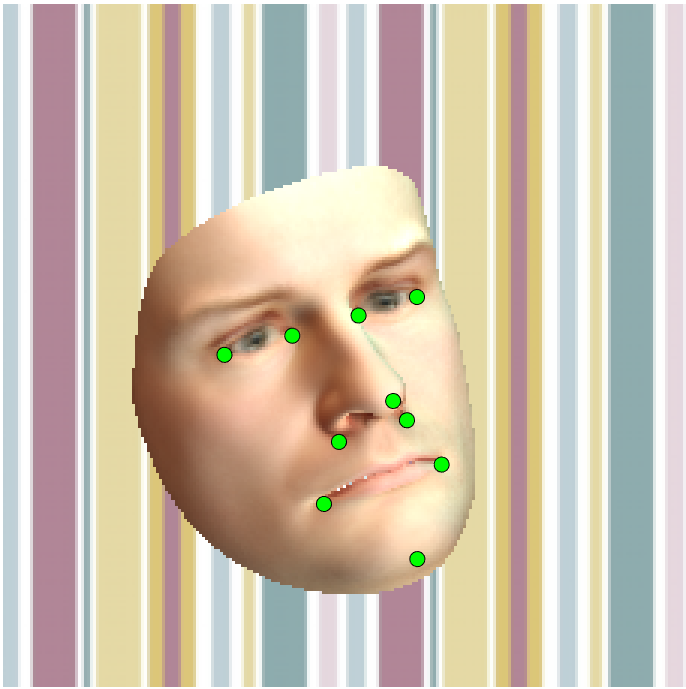
\includegraphics[width=0.3\textwidth]{Figures/chap3/original_all_lms.png}}\hfill
	\subbottom[The same image as in (a) but with an occlusion and two underlying landmarks which are disabled because they're not visible anymore.]{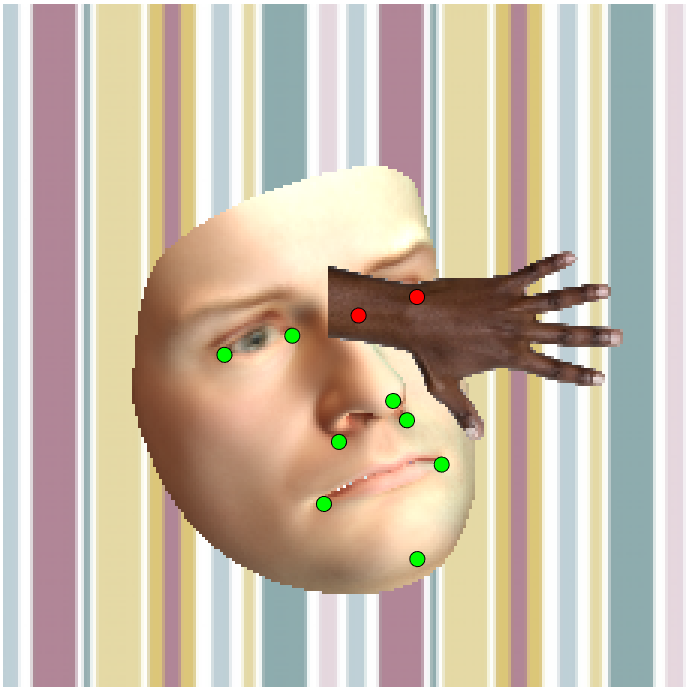
\includegraphics[width=0.3\textwidth]{Figures/chap3/occluded_parts_lms.png}}
	\hspace*{\fill}%
	\caption{Because of the occlusion, certain landmarks had to be disabled. The image shows original landmarks (green dots) and the landmark which had to be deactivated (red dots).}
	\label{appendix:lms}
\end{figure}

The software provides csv-files, rps-files, tlms-files, ground truth masks, images with occlusions and images without occlusions for both the 'bfm' version and for the tailored 'face12' version of the Basel Face Model. If an occlusion gets rendered over a landmark, it gets disabled.